% file: 3-11-matchings-factors/chinese-postman-problem-edge-disjoint.tex

\documentclass[tikz]{standalone}
\usetikzlibrary{positioning, decorations.pathmorphing}

\begin{document}
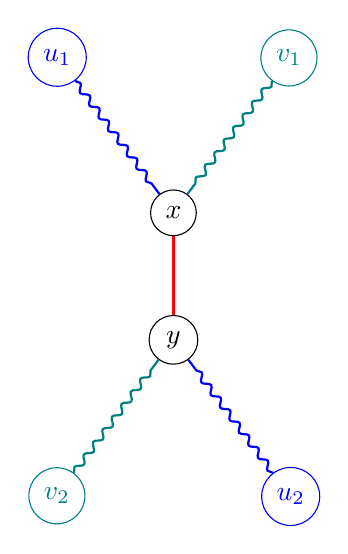
\begin{tikzpicture}[every node/.style = {draw, circle, minimum size = 15pt},
  node distance = 1.5cm and 1.0cm,
  path/.style = {thick, -, decorate, decoration = {snake, amplitude = .4mm, segment length = 2mm, post length = 1mm}}]
  \node (x) [] {$x$};
  \node (y) [below = 1.0cm of x] {$y$};

  \node (u1) [blue, above left = of x] {$u_1$};
  \node (u2) [blue, below right = of y] {$u_2$};
  \node (v1) [teal, above right = of x] {$v_1$};
  \node (v2) [teal, below left = of y] {$v_2$};

  \path (x) edge[red, very thick] (y)
  	(u1) edge[blue, path] (x)
	(v1) edge[teal, path] (x)
	(u2) edge[blue, path] (y)
	(v2) edge[teal, path] (y);
\end{tikzpicture}
\end{document}